\chapter{Foundations}

\section{Definition of Trace Link Recovery}
Traceability is the ability for something to be traced. Meaning, there is evidence of some past occurrence. %Do I need to quote a dictionary here?
The task of trace link recovery (TLR) in software engineering is to find instances of the same element across different artifacts and link them for further processing. These traceability links help with tracking relationships between for example: code, requirements, diagrams, documentation, \dots

This becomes especially important when inconsistencies are introduced into the project's artifacts. 

As shown by \citewithauthor{wohlrab2019ImprovingConsistency} inconsistency in wording and language is quite common during different stages of development. For example, naming conventions for architectural components may not be followed during implementation. They find the impact of these inconsistencies to be quite insignificant. However, for trace link recovery, this means that simple string comparisons by name are insufficient.



\section{Definition of Automated Prompt Engineering}
Prompt engineering is the process of refining a prompt for the specific use case. This is usually done in a non-systematic manual way. Automated Prompt Engineering (APE) enables Large Language Models to refine the initial prompt in order to optimize its performance \cite{zadenoori2025AutomaticPrompt}. 

Typically, automatic prompt engineering processes are iterated to improve previous results further\citeiterative . The performance of prompts can be measured using a set of training data, which includes input/output pairs. 

\subsection{Initial Prompt}
The initial prompt will be the origin for the refinement process. It needs to be selected firstly before any optimization can occur. This prompt can be chosen manually. This approach is very intuitive, however manual human interaction is still required to design this initial prompt. 

\citewithauthor{zhou2023LargeLanguage} propose using the LLM to generate the initial prompt. They prompt the model to generate a likely set of instructions, also called candidates, that will achieve good results with a batch of input/output pairs.




\section{Automatic Prompt Optimization Using Gradient Descent}
\label{sec:gradient_descent}
Based on the work of \citewithauthor{pryzant2023AutomaticPrompt} I will implement a more sophisticated prompt optimization algorithm into the LiSSA framework. They propose the Prompt Optimization with Textual Gradients (ProTeGi) algorithm. This entire section is based on their work.

The ProTeGi algorithm takes an initial prompt $p_0$ and training data $\{(x_1, y_1), \dots, (x_n, y_n)\}$ consisting of input and output. They \directQuote[sec. 2]{assume access to a black box LLM API [...] which returns a likely text continuation y of the prompt formed by concatenating p and x}{pryzant2023AutomaticPrompt}. They then iteratively optimize the initial prompt $p_0$ to produce an approximation of the most optimized prompt for the given task. In order to optimize the prompt, a function is required, to compute deviance between the actual output $y$ and expected output $y_i$ as a numeric value.

\begin{figure}[h]
\centering
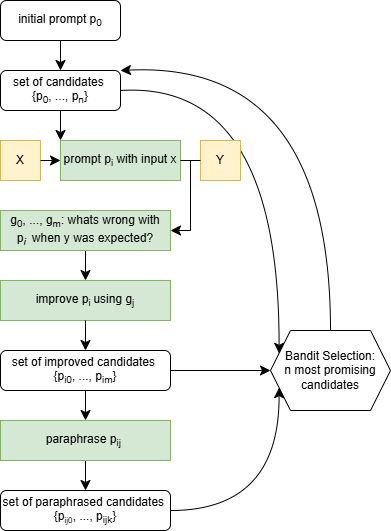
\includegraphics[width=9cm]{graphics/gradient_descent.png}
\caption{Overview of the iterative optimization loop in \cite{pryzant2023AutomaticPrompt}}
\label{fig:gradient_descent}
TODO: 
\begin{itemize}
    \item improve resolution
    \item add legend
    \item symbolise core loop
\end{itemize}
\end{figure}


\subsectoion{Evaluation and Expansion}
To evaluate the output of the current prompt $p_i$, they use a loss signal prompt $\triangledown$. In addition to the prompt errors that were not correctly classified when testing $p_i$ are also provided. The result summarizes the flaws of $p_i$ in natural language. This summary is called the textual gradient $g$.

The second prompt $\delta$ they use, is required to adjust $p_i$ in the opposite direction of $g$ to minimize the loss signal. They differ from other implementations by generating multiple gradients and refinements that might improve $p_i$ and select good candidates to optimize further in the next iterative step.

In addition, they broaden their candidates further by paraphrasing them into semantically similar prompts, which are worded different. Generating new prompts with $g$ and broadening them is considered candidate expansion.

\subsection{Candidate Selection}
In order to select candidates for the next iteration, they apply a beam search algorithm. Beam search is a heuristic best first graph search algorithm to select a fixed number of promising paths. The remaining paths will be discarded to allocate resources on more promising paths instead. \cite{BeamSearch}

The selection of the most promising candidates is quite expensive on the training set. As the problem is quite similar to the best arm identification in bandit optimization by \citewithauthor{audibert2010BestArm}, they rely on this well studied problem instead.

The problem consists of $N$ stochastically independent probability distributions $\{ D_1, \dots, D_N\}$ with corresponding expected values and variances. These distributions are unknown to the user initially. The goal is to maximize the sum of rewards for each pull from the set of probability distributions, utilizing the knowledge gained through previous pulls. \cite{kuleshov2014AlgorithmsMultiarmeda}

It is an analogy to multiple one-armed bandit slot machines. Pulling a lever on one of these slot machines does not affect the others but costs noticeable resources. The optimization aims to find the best performing arms with as few pulls as possible. 

\citeauthor{pryzant2023AutomaticPrompt} have used the successive rejects algorithm by \citewithauthor{audibert2010BestArm} to select the best prompt candidates for the next iteration step.

The set of current candidates $S$ is therefore initialized with all $k$ candidate prompts in the iteration step. Depending on the budget for sampling candidates and remaining candidates in $S$ will be prompted with $n_k$ pairs of the training data. The results are evaluated with a metric function $m$ to quantify the performance. The lowest scoring prompt is discarded from $S$ and sampling repeated with the remainder until the set $S$ only contains the desired amount of candidates.

The remaining candidates will be used as initial prompts for the next expansion step.

\textit{TODO: Explain successive rejects}

\begin{algorithm}
\caption{\directQuote[Algorithm 4, p. 4]{$Select(\cdot)$ with Successive Rejects}{pryzant2023AutomaticPrompt}}
\begin{algorithmic}[1]
    \State Initialize: $S_0 \gets \{p_1, \dots , p_n\}$
    \For{$k = 1, \dots , {n − 1}$}
        \State Sample $D_{sample} \subset D_{tr}, |D_{sample}| = n_k$
        \State Evaluate $p_i \in S_{k−1}$ with $m(p_i, D_{sample})$
        \State $S_k \gets S_{k−1}$, excluding the prompt with the lowest score from the previous step
    \EndFor
    \State \Return Best prompt $p^* \in S_{n-1}$
\end{algorithmic}
\end{algorithm}


\textit{Three Pages}